\documentclass[11pt]{article}

\usepackage[letterpaper,margin=0.75in]{geometry}
\usepackage{booktabs}
\usepackage{graphicx}
\usepackage{listings}

\setlength{\parindent}{1.4em}

\begin{document}

\lstset{
  language=Python,
  basicstyle=\small,          % print whole listing small
  keywordstyle=\bfseries,
  identifierstyle=,           % nothing happens
  commentstyle=,              % white comments
  stringstyle=\ttfamily,      % typewriter type for strings
  showstringspaces=false,     % no special string spaces
  numbers=left,
  numberstyle=\tiny,
  numbersep=5pt,
  frame=tb,
}

\title{Reliable Transport}

\author{Jonathan George}

\date{}

\maketitle

\section{Description}
For this project, we have implemented a reliable transport protocal based on TCP. The major components of this protocal include a sender window buffer, receiver acknowledment, and a resend timer. 
In this protocal, the sender first places all the data to send into a buffer. This buffer has a sliding window which keeps track of packets unsent, sent and acknowledged. 
The sender upon starting to send a packet will send all availible packets allowed by the window size. It will not send a packet which is more than the window size away from the lowest unacknowledged packet.
Whenever the receiver recieves a packet, it will store this packet in a buffer and sent an ack for the lowest segment it needs next. The receiver will store packets which are out of order, so if a single segment is missing it will catch itself up once it recieves that segment.
When the sender receives an ack for a message it will tell the buffer to slide the window to that ack number and send any newly made availible data within the new window space. 
The resend timer is reset everytime a packet is sent from the reciever side. It plays the role of a watchdog timer, watching for a dropped packet or too slow of a connection. When it expires, it will resend the lowest unacknowledged packet and wait again for a returning ack. When this ack arrives the sender will send all data availible based on that ack.

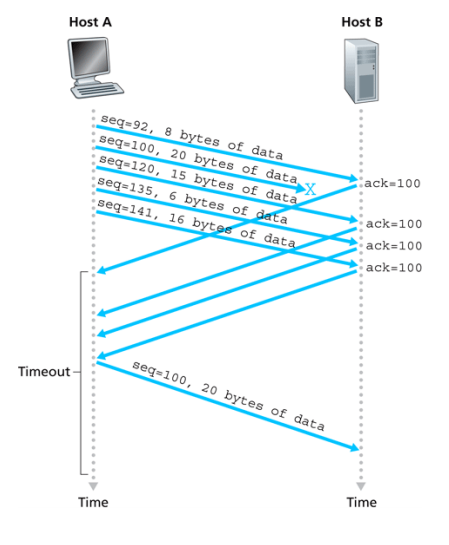
\includegraphics[width=11cm]{fast_transport.png}

Credit for image is given to Dr. Zappala's class slides.

\section{Tests}
In this section, we will describe the tests we used to test our TCP implementation. These tests were checked by using transfer.py which was provided by Dr. Zappala. This test script accepts a window size, file and loss rate in order to test different scenerios. Each test was using a two node scenerio found in networks/one-hop.txt.



Test Cases:
\begin{enumerate}
\item Bandwidth of 10Mbps, propegation delay of 10ms and window size of 3000 bytes. Transferring test.txt.
\begin{enumerate}
\item loss rate of 0\%. Took 0.0732 seconds
\item loss rate of 10\%. Took 1.0732 seconds
\item loss rate of 20\%. Took 3.0948 seconds
\item loss rate of 50\%. Took 14.0732 seconds
\end{enumerate}

\item Bandwidth of 10Mbps, propegation delay of 10ms and window size of 3000 bytes. Transferring internet-architecture.pdf.
\begin{enumerate}
\item loss rate of 0\%. Took 1.07 seconds
\item loss rate of 10\%. Took 32 seconds
\item loss rate of 20\%. Took 64 seconds
\item loss rate of 50\%. Took 359 seconds
\end{enumerate}

\end{enumerate}

The total time the test takes in each of these cases depends on the random element of packet loss, but it is clear the the one second timeout is insuficent, since it means there is time spent waiting for the timer to expire when no packets are on the network. This leads us to implementing a dynamic timer.

\section{Dynamic Retransmission Timer}

The Dynamic timer is implemented by estimating RTT (Round Trip Time) and using an exponential backoff function to slowly approach the proper value. Packet loss indicates the RTT estimate is too low. Therefore when the transmission timer expires, it doubles the RTT in order to compensate for this. 
Each time an ack is recieved the timer value is updated by the following equation:

NewEstimatedRTT = (1 − alpha) ∗ OldEstimatedRTT + alpha ∗ SampleRTT 

In our implementation we chose alpha to equal 1/8. 

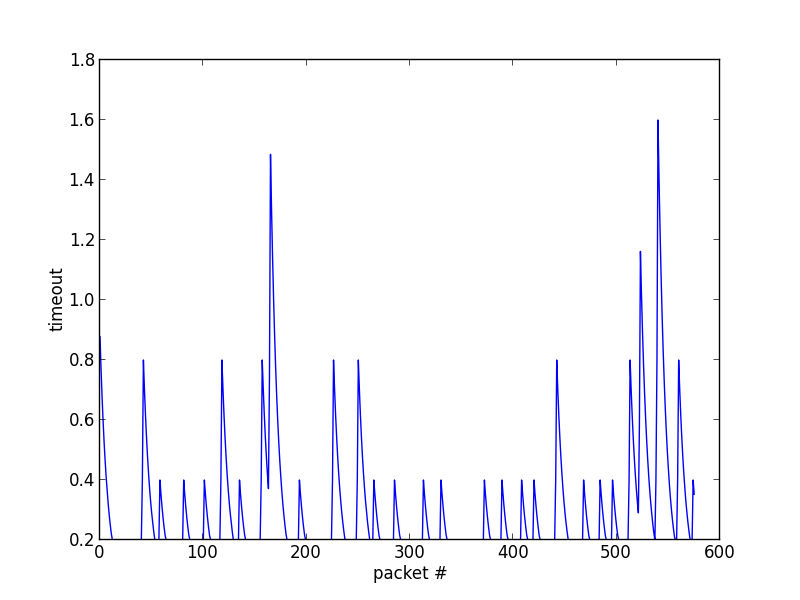
\includegraphics[width=11cm]{timeout.png}

This graph shows the exponential backoff of the timeout value when packets are reliable and the doubling of the timeout value when a packet is lost. 

\section{Experiments}
In this section, we explore the effects of window size on the throughput and queuing delay when there is a loss rate of 0\%

We set up a two node network setup with a bandwidth of 10 Mbps, a propagation delay of 10 ms, a queue size of 100 and a loss rate of 0\%. We transferred the internet-architecture.pdf file using window sizes of 1000, 2000, 5000, 10000, 15000, and 20000 bytes. We then computed the throughput of the transfer as the total bits sent divided by the total time to send the file and the average queueing delay of all segments sent. 



Throughput vs Window Size:

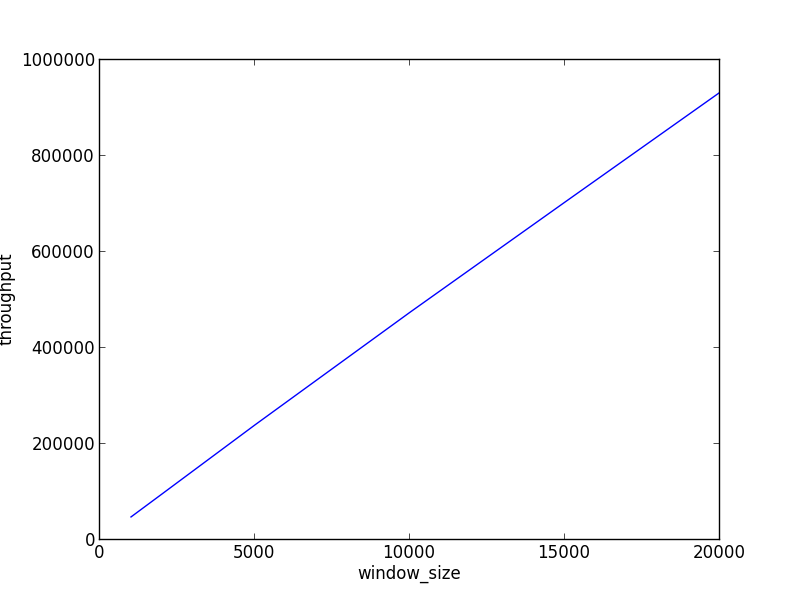
\includegraphics[width=11cm]{throughput.png}

Queueing Delay vs Window Size:

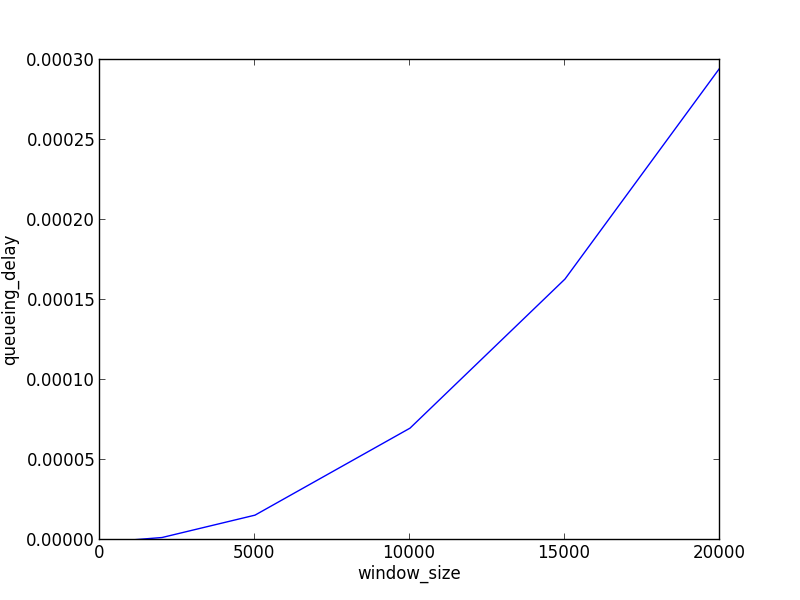
\includegraphics[width=11cm]{queueing_delay.png}

As can be seen by the graph, the throughput increases linearly as you increase the window size. However, the queuing delay increases exponentially. This will require us to implement conguestion control in the next lab. 

\section{Source Code}

Source code for this report can be found at https://github.com/qzcx/bene

\end{document}
